\documentclass[table,hyperref={bookmarksopen=false}]{beamer}

\usepackage[utf8]{inputenc} % encoding of latex files
\usepackage[ngerman]{babel} % language hyphenation

% for pgf images in beamer template
\usepackage{pgf}

% used for special math symbols and environments such as align
\usepackage{amsmath}
\usepackage{amssymb}
\usepackage{etex}


% graphics
\usepackage{graphicx} % for graphics
% \graphicspath{{images/}} % path for graphics

% for bibliography using biblatex
% \usepackage[style=verbose,hyperref=false,backref=false]{biblatex} % define style and used options of biblatex
% \usepackage[babel,german=quotes]{csquotes} % define quotes
% \bibliography{include/bibliography} % path to bib file

\usetheme[section]{tubs}

%\setbeamertemplate{itemize items}[ball]
%\setbeamertemplate{itemize items}[square]
\setbeamertemplate{itemize items}[tusquare]

\title{Ein Beamertheme für das neue Corporate Design}
\subtitle{Beispiel und Anleitung}
\author[Jens Brandt]{\underline{Jens Brandt}, ggf. weitere Autoren}
\institute[TU Braunschweig, IBR]{Technische Universität Braunschweig, IBR}

\date{Name der Konferenz oder einfach nur ein Datum}

\logo{\includegraphics{ibr_deu}}
%\titlegraphic{iz}
\titlegraphic{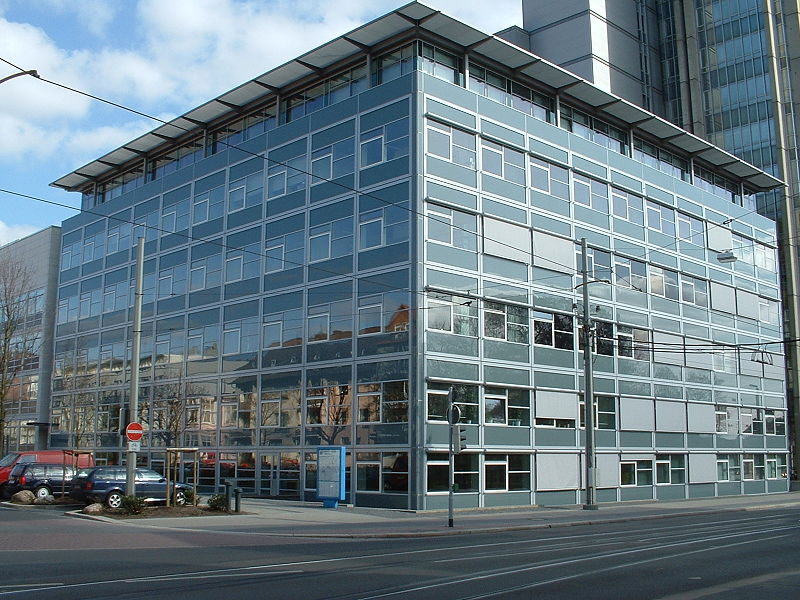
\includegraphics{infozentrum.jpg}}



\begin{document}

\frame[plain]{\titlepage}

\setbeamercolor{frametitle}{fg=white,bg=tuRed}
\frame{
        \frametitle{Outline}
        \tableofcontents
        }
\setbeamercolor{frametitle}{fg=black,bg=tuGrey}


\section{Introduction}

\frame{
 \frametitle{Introduction}
 \begin{block}{Scope}
 \begin{itemize}
     \item A new theme for beamer
 \end{itemize}
 \end{block}
 \begin{block}{Problem}
    \begin{itemize}
        \item How to emulate the original layout?
    \end{itemize}
 \end{block}
 \begin{block}{Approach}
     \begin{itemize}
         \item Create a beamertheme that is better than the PPT template ;-)
     \end{itemize}
 \end{block}
}

\section{Introduction}

\frame{
 \frametitle{Introduction}
 \begin{enumerate}
   \item Fußnoten-Test\footnote{Dies ist eine Fußnote die nicht hinter dem Logo verschwindet.}
 \end{enumerate}

}

\section{Theme}

\frame{
  \frametitle{Dateien}
  \begin{itemize}
    \item {\tt beameroutlinetheme.sty}: Das Beamer Theme
    \item {\tt tu-logo-new.pdf}: Das neue TU Logo als Vektorgrafik
    \item {\tt altbau.jpg}: Foto des Altbaus für die Titelfolie (Default)
    \item {\tt iz.jpg}: Foto des Informatikzentrums für die Titelfolie
  \end{itemize}
}

\begin{frame}[fragile]
  \frametitle{Benutzung}
  Theme einstellen:
  \begin{verbatim}
    \useoutertheme[relax,section]{tubs}
  \end{verbatim}
  \begin{block}{Optionen}
  \begin{itemize}
    \item relax: verkleinert den weißen unteren Rand im Vergleich zur PPT Vorlage
    \item section: zeigt die section Überschriften am oberen Rand der Frames an
  \end{itemize}
  \end{block}
\end{frame}

\begin{frame}[fragile]
  \frametitle{Besondere Folien}
  \begin{block}{Titelfolie}
  \begin{verbatim}
    \frame[plain]{\titlepage}
  \end{verbatim}
  \end{block}
  \begin{block}{Outline}
  \begin{verbatim}
    \setbeamercolor{frametitle}{fg=white,bg=tuRed}
    \frame{
              \frametitle{Outline}
              \tableofcontents
    }
    \setbeamercolor{frametitle}{fg=black,bg=tuGrey}
  \end{verbatim}
  \end{block}
\end{frame}

\begin{frame}[fragile]
  \frametitle{Itemize}
  \begin{block}{Default}\vspace*{-3mm}
  \begin{verbatim}
    \setbeamertemplate{itemize items}[tusquare]
  \end{verbatim}\vspace*{-3mm}
  \begin{itemize}
    \item Erste Ebene
    \begin{itemize}
      \item Zweite Ebene
      \begin{itemize}
        \item Dritte Ebene
      \end{itemize}
    \end{itemize}
  \end{itemize}
  \end{block}
  \begin{block}{Alternativ}\vspace*{-3mm}
  \begin{verbatim}
    \setbeamertemplate{itemize items}[ball]
  \end{verbatim}\vspace*{-3mm}
  \setbeamertemplate{itemize items}[ball]
  \begin{itemize}
    \item Erste Ebene
    \begin{itemize}
      \item Zweite Ebene
      \begin{itemize}
        \item Dritte Ebene
      \end{itemize}
    \end{itemize}
  \end{itemize}
  \end{block}
\end{frame}


\begin{frame}[fragile]
  \frametitle{Itemize (cont.)}
  \begin{block}{Oder auch}\vspace*{-3mm}
  \begin{verbatim}
    \setbeamertemplate{itemize items}[square]
  \end{verbatim}\vspace*{-3mm}
  \setbeamertemplate{itemize items}[square]
  \begin{itemize}
    \item Erste Ebene
    \begin{itemize}
      \item Zweite Ebene
      \begin{itemize}
        \item Dritte Ebene
      \end{itemize}
    \end{itemize}
  \end{itemize}
  \end{block}
  Der Aufzählungstyp kann einmalig zu Beginn oder an beliebiger Stelle gesetzt werden. Somit ist auch ein Wechsel des Typs innerhalb der Präsentation möglich.
\end{frame}

\begin{frame}[fragile]
  \frametitle{Enumerate}
  \begin{block}{Default}
  \begin{enumerate}
    \item Erste Ebene
    \begin{enumerate}
      \item Zweite Ebene
      \begin{enumerate}
        \item Dritte Ebene
      \end{enumerate}
    \end{enumerate}
  \end{enumerate}
  \end{block}
  \begin{block}{Alternativ}\vspace*{-3mm}
  \begin{verbatim}
    \setbeamertemplate{enumerate items}[ball]
  \end{verbatim}\vspace*{-3mm}
  \setbeamertemplate{enumerate items}[ball]
  \begin{enumerate}
    \item Erste Ebene
    \begin{enumerate}
      \item Zweite Ebene
      \begin{enumerate}
        \item Dritte Ebene
      \end{enumerate}
    \end{enumerate}
  \end{enumerate}
  \end{block}
\end{frame}


\begin{frame}[fragile]
  \frametitle{Grafiken}
  Optional kann ein Instituts- oder Projektlogo angegeben werden, das auf der Titelfolien oben rechts und auf den anderen Folien unten rechts angezeigt wird.
  Das Logo wird auf eine feste Höhe skaliert.
  \begin{verbatim}
    \instlogo{ibr_deu}
  \end{verbatim}
  Ohne weitere Angabe wird auf der Titelfolie das Foto des Altbaus gezeigt. Dieses Foto kann durch eine beliebige Grafik ersetzt werden, die entsprechend skaliert wird. Daher sollte die Grafik ein Seitenverhältnis von 1:3.219 haben,
  \begin{verbatim}
    \titlegraphic{iz}
  \end{verbatim}
  In beiden Fällen kann der Dateiname mit oder ohne Endung angegeben werden.
\end{frame}

\begin{frame}[fragile]
  \frametitle{Besonderheiten}
  Der graue Kasten am oberen Rand wird nur erzeugt, wenn ein Titel für den Frame angegeben wurde.
  \begin{verbatim}
    \frametitle{Titel}
  \end{verbatim}
  Andernfalls siehe nächste Folie ...
\end{frame}

\section{Conclusion}

\frame{
    \begin{center}
      {\textbf{\LARGE Questions?}} \\[5mm]
    Jens Brandt\\[0mm]
    \tt{brandt@ibr.cs.tu-bs.de}
    \end{center}
    }
        
\end{document}

